\documentclass[11pt,letterpaper]{article}
\usepackage[T1]{fontenc}
\usepackage[scaled]{helvet}
\renewcommand{\familydefault}{\sfdefault}
\usepackage{amsmath,amssymb}
\usepackage[margin=0.8in,bottom=0.9in]{geometry}
\usepackage[most]{tcolorbox}
\usepackage{tikz}
\usetikzlibrary{calc}
\usepackage{enumitem}
\usepackage{array}
\usepackage{needspace}
\usepackage{fancyhdr}
\usepackage{pifont}

% ---- Palette "F. Bright & Playful" ----
\definecolor{fmtitle}{HTML}{3D2C8D}
\definecolor{fmkey}{HTML}{0096C7}
\definecolor{fmwatch}{HTML}{2BB673}
\definecolor{fmturn}{HTML}{F4A100}
\definecolor{fmmistake}{HTML}{EF476F}
\definecolor{fmnotice}{HTML}{9B5DE5}
\definecolor{fmgray}{HTML}{6B6B6B}

\pagestyle{fancy}
\fancyhf{}
\renewcommand{\headrulewidth}{0pt}
\fancyfoot[C]{\footnotesize\color{fmgray}\textcopyright\ 2026 FangMath. All rights reserved.}
\fancyfoot[R]{\footnotesize\color{fmgray}\thepage}
\setlength{\parindent}{0pt}
\setlength{\parskip}{3pt}

\newcommand{\badge}[1]{\colorbox{fmtitle}{\color{white}\bfseries\small\ #1\ }}
\newcommand{\leveltag}[2]{\colorbox{#1}{\color{white}\bfseries\scriptsize\ #2\ }}
\newcommand{\LE}{\leveltag{fmwatch}{EASY}}
\newcommand{\LM}{\leveltag{fmturn}{MEDIUM}}
\newcommand{\LH}{\leveltag{fmmistake}{HARD}}

\newcommand{\sectionbar}[2]{\needspace{6cm}\par\vspace{4mm}
  \begin{tcolorbox}[enhanced,colback=fmtitle,colframe=fmtitle,arc=2mm,
    left=4mm,top=1.5mm,bottom=1.5mm]
  \color{white}\bfseries\large #1\hfill{\normalsize\mdseries #2}
  \end{tcolorbox}}

\newtcolorbox{keyidea}{enhanced,breakable,colback=white,colframe=fmkey,boxrule=1pt,arc=2mm,
  title={Key Idea},coltitle=fmkey,fonttitle=\bfseries,
  attach boxed title to top left={xshift=4mm,yshift=-2mm},
  boxed title style={colback=white,colframe=fmkey,boxrule=0.9pt}}
\newtcolorbox{watchme}{enhanced,colback=white,colframe=fmwatch,boxrule=1pt,arc=2mm,
  title={Watch Me --- Worked Example},coltitle=fmwatch,fonttitle=\bfseries,
  attach boxed title to top left={xshift=4mm,yshift=-2mm},
  boxed title style={colback=white,colframe=fmwatch,boxrule=0.9pt}}
\newtcolorbox{mistakebox}{enhanced,breakable,colback=white,colframe=fmmistake,boxrule=1pt,arc=2mm,
  title={Common Mistake},coltitle=fmmistake,fonttitle=\bfseries,
  attach boxed title to top left={xshift=4mm,yshift=-2mm},
  boxed title style={colback=white,colframe=fmmistake,boxrule=0.9pt}}
\newtcolorbox{yourturn}{enhanced,breakable,colback=white,colframe=fmturn,boxrule=1pt,arc=2mm,
  title={Your Turn},coltitle=fmturn,fonttitle=\bfseries,
  attach boxed title to top left={xshift=4mm,yshift=-2mm},
  boxed title style={colback=white,colframe=fmturn,boxrule=0.9pt}}
\newtcolorbox{answerbox}[1]{enhanced,breakable,colback=white,colframe=fmwatch,boxrule=1pt,arc=2mm,
  title={#1},coltitle=fmwatch,fonttitle=\bfseries,
  attach boxed title to top left={xshift=4mm,yshift=-2mm},
  boxed title style={colback=white,colframe=fmwatch,boxrule=0.9pt}}

\newcommand{\work}[1]{\par\vspace{#1}}
\setlist[enumerate]{itemsep=2pt,topsep=3pt}

% ---------------- extra boxes ----------------
\newtcolorbox{notebox}{enhanced,breakable,colback=white,colframe=fmnotice,boxrule=1pt,arc=2mm,
  title={Notice},coltitle=fmnotice,fonttitle=\bfseries,
  attach boxed title to top left={xshift=4mm,yshift=-2mm},
  boxed title style={colback=white,colframe=fmnotice,boxrule=0.9pt}}
\newtcolorbox{exbox}{enhanced,colback=white,colframe=fmwatch,boxrule=0.8pt,arc=2mm,
  title={Example},coltitle=fmwatch,fonttitle=\bfseries\small,
  attach boxed title to top left={xshift=4mm,yshift=-2mm},
  boxed title style={colback=white,colframe=fmwatch,boxrule=0.8pt},fontupper=\small}
\newcommand{\topicbar}[1]{\needspace{4.5cm}\par\vspace{5mm}
  \begin{tcolorbox}[enhanced,colback=fmtitle,colframe=fmtitle,arc=2mm,left=4mm,top=1.5mm,bottom=1.5mm]
  \color{white}\bfseries\large #1
  \end{tcolorbox}}
\usepackage{multicol}

% ---------------- practice layout ----------------
\newcommand{\workline}{\par\vspace{7mm}{\color{gray!55}\rule{\linewidth}{0.4pt}}}
\newcommand{\worklines}[1]{\foreach \i in {1,...,#1}{\workline}}
\newcommand{\prob}[3]{\needspace{#3}\par\vspace{3mm}{\color{fmturn}\bfseries #1.}\ #2\par}
\newcommand{\ansline}{\par\vspace{4mm}\hfill\textbf{Answer:}\ \rule{5cm}{0.4pt}\par}
\newcommand{\keyitem}[3]{\needspace{3.2cm}\par\vspace{2mm}
  \begin{tcolorbox}[enhanced,colback=white,colframe=fmwatch!60,boxrule=0.6pt,arc=1.5mm,left=3mm,top=1.5mm,bottom=1.5mm]
  {\color{fmwatch}\bfseries #1.}\quad\small #2\par\vspace{1mm}
  \normalsize\textbf{Answer: #3}
  \end{tcolorbox}}


\usetikzlibrary{arrows.meta}
\providecommand{\iskey}{0}
% fill-in blank: line for students, pink answer in the key
\newcommand{\fb}[2][2.6cm]{\ifnum\iskey=1 \underline{\makebox[#1][c]{\color{fmmistake}\bfseries #2}}\else\underline{\makebox[#1]{}}\fi}
% answer line for practice problems
\newcommand{\pans}[2][3.2cm]{\ifnum\iskey=1 \underline{\makebox[#1][c]{\color{fmmistake}\bfseries #2}}\else\rule{#1}{0.4pt}\fi}
\newcommand{\vid}[1]{{\color{fmgray}\small\textit{\ding{43} Video: #1}}}
\newcommand{\pt}[2]{\fill (#1) circle (2.2pt) node[above=1pt,font=\small]{$#2$};}

\usetikzlibrary{decorations.pathreplacing}

\begin{document}
\ifnum\iskey=1 \colorbox{fmwatch}{\color{white}\bfseries\small\ ANSWER KEY\ }\else\badge{WATCH \& FILL IN}\fi\hfill{\small\color{fmgray}Geometry \textperiodcentered\ Lesson 1.2}\par\vspace{4mm}
{\color{fmtitle}\LARGE\bfseries Segment Addition Postulate --- Notes\ifnum\iskey=1 \ --- Answer Key\fi}\par\vspace{1mm}
{\color{fmgray}Watch the video and fill in each blank. Pause when you see ``Your turn.''}\par\vspace{3mm}
Name: \rule{6cm}{0.4pt}\hspace{1cm}Date: \rule{3.5cm}{0.4pt}\par\vspace{2mm}

\vid{Walk 4 steps, then 7 more}
\begin{keyidea}\begin{minipage}[c]{0.55\linewidth}\centering
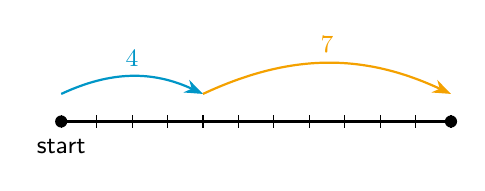
\begin{tikzpicture}[x=0.45cm]
\draw[thick] (0,0)--(11,0);\foreach \i in {0,...,11} \draw (\i,-0.08)--(\i,0.08);
\fill (0,0) circle(2.2pt) node[below=3pt,font=\small]{start};
\draw[fmkey,thick,-{Stealth}] (0,0.35) to[bend left=25] node[above,font=\small]{$4$} (4,0.35);
\draw[fmturn,thick,-{Stealth}] (4,0.35) to[bend left=25] node[above,font=\small]{$7$} (11,0.35);
\fill (11,0) circle(2.2pt);
\end{tikzpicture}\end{minipage}\hfill
\begin{minipage}[c]{0.42\linewidth}Walk $4$, then $7$ more.\par\vspace{1mm}
Distance from the start: \ $4 + 7 = $ \fb[1.2cm]{$11$}\end{minipage}\end{keyidea}

\vid{The postulate}
\begin{keyidea}\begin{center}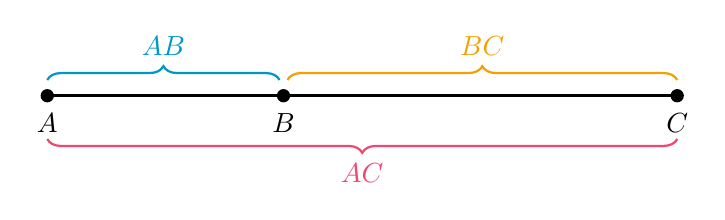
\begin{tikzpicture}[x=1cm]
\draw[very thick] (0,0)--(8,0);
\fill (0,0) circle(2.4pt) node[below=3pt]{$A$} (3,0) circle(2.4pt) node[below=3pt]{$B$} (8,0) circle(2.4pt) node[below=3pt]{$C$};
\draw[fmkey,thick,decorate,decoration={brace,amplitude=5pt}] (0,0.2)--(2.95,0.2) node[midway,above=5pt]{$AB$};
\draw[fmturn,thick,decorate,decoration={brace,amplitude=5pt}] (3.05,0.2)--(8,0.2) node[midway,above=5pt]{$BC$};
\draw[fmmistake,thick,decorate,decoration={brace,amplitude=5pt,mirror}] (0,-0.55)--(8,-0.55) node[midway,below=5pt]{$AC$};
\end{tikzpicture}\end{center}
\textbf{Segment Addition Postulate:} If $B$ is \fb[2cm]{between} $A$ and $C$, then \ \fb[3.4cm]{$AB + BC = AC$}.\par\vspace{2mm}
In words: \ part $+$ part $=$ \fb[1.8cm]{whole}.\end{keyidea}

\vid{Simple cases first}
\begin{keyidea}\begin{minipage}[t]{0.47\linewidth}\textbf{Find the whole:} \fb[1.6cm]{add}\par\vspace{1mm}
$AB = 4,\ BC = 7$\par\vspace{1mm}
$AC = AB + BC = 4 + 7 = $ \fb[1.2cm]{$11$}\end{minipage}\hfill
\begin{minipage}[t]{0.47\linewidth}\textbf{Know the whole and one piece:} \fb[1.8cm]{subtract}\par\vspace{1mm}
$AC = 20,\ AB = 8$\par\vspace{1mm}
$BC = AC - AB = 20 - 8 = $ \fb[1.2cm]{$12$}\end{minipage}\end{keyidea}

\vid{With algebra}
\begin{watchme}$AB = x + 3,\quad BC = 2x,\quad AC = 21.$ \ Find $x$ and $BC$.\par\vspace{2mm}
\renewcommand{\arraystretch}{1.7}\begin{tabular}{@{}l l@{}}
$(x + 3) + 2x = 21$ & part $+$ part $=$ \fb[1.4cm]{whole}\\
\fb[2.2cm]{$3x + 3$} $= 21$ & combine like terms\\
$3x = $ \fb[1.2cm]{$18$} & subtract 3\\
$x = $ \fb[1.2cm]{$6$} & \textbf{don't stop at $x$!}\\
$BC = 2(6) = $ \fb[1.2cm]{$12$} & answer the question they asked\\
Check: $AB = $ \fb[1cm]{$9$}, \ $9 + 12 = 21$ \ \ding{51} & \\
\end{tabular}\end{watchme}

\vid{Only when $B$ is between $A$ and $C$}
\begin{mistakebox}\begin{minipage}[c]{0.3\linewidth}\centering
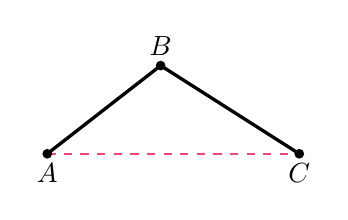
\begin{tikzpicture}[scale=0.8]\draw[very thick] (0,0)--(1.8,1.4)--(4,0);\draw[thick,dashed,fmmistake] (0,0)--(4,0);
\fill (0,0) circle(2.2pt) node[below]{$A$} (1.8,1.4) circle(2.2pt) node[above]{$B$} (4,0) circle(2.2pt) node[below]{$C$};\end{tikzpicture}\end{minipage}\hfill
\begin{minipage}[c]{0.66\linewidth}The postulate only works when $B$ is \fb[1.8cm]{between} $A$ and $C$ on one line.\par\vspace{1mm}
If $A$, $B$, $C$ make a triangle, then $AB + BC$ is \fb[1.6cm]{more} than $AC$.\end{minipage}\end{mistakebox}

\vid{Your turn}
\begin{yourturn}$Q$ is between $P$ and $R$. \quad $PQ = 3x - 1,\quad QR = x + 5,\quad PR = 24.$ \ Find $x$ and $PQ$.\par\vspace{2mm}
$(3x - 1) + (x + 5) = 24$\par\vspace{1mm}
\fb[2.2cm]{$4x + 4$} $= 24$ \quad $\Rightarrow$ \quad $x = $ \fb[1.2cm]{$5$}\par\vspace{1mm}
$PQ = 3(5) - 1 = $ \fb[1.2cm]{$14$} \qquad Check: $QR = $ \fb[1cm]{$10$}, \ $14 + 10 = 24$ \ding{51}\end{yourturn}

\begin{notebox}\textbf{Remember:}\quad \textbf{part $+$ part $=$ whole} ($AB + BC = AC$ when $B$ is between $A$ and $C$).\quad Missing piece? \textbf{Subtract} from the whole.\quad Solve for $x$ --- then answer the question they actually asked.\end{notebox}
\end{document}
